\documentclass[article]{stucosrec}

% for testing purposes only
\usepackage{lipsum}
\newcommand{\latex}{\LaTeX\xspace}

\title{\latex TEMPLATE FOR StuCoSReC CONTRIBUTION}
\author{
	Klemen Berkovi\v{c}\thanks{He did the most work} \\
	Faculty of Electrical \\Engineering and Computer Science,\\
	University of Maribor,\\
	Koro\v{s}ka cesta 46, 2000 Maribor, Slovenia \\
	\texttt{klemen.berkovic1@um.si}
	\And
	Iztok Fister Jr.\thanks{The best sponsor of them all} \\
	Faculty of Electrical \\Engineering and Computer Science,\\
	University of Maribor,\\
	Koro\v{s}ka cesta 46, 2000 Maribor, Slovenia \\
	\texttt{iztok.fister1@um.si}
	\AND
	Iztok Fister \thanks{He is the boss} \\
	Faculty of Electrical \\Engineering and Computer Science,\\
	University of Maribor,\\
	Koro\v{s}ka cesta 46, 2000 Maribor, Slovenia \\
	\texttt{iztok.fister@um.si}
}

% images directory
\imagespath{ {./images/} }

\begin{document}
	
	\maketitle
	
	\begin{abstract}
		This paper provides a sample of a \latex document which
conforms to the formatting guidelines for StuCosRec Proceedings.
		It is a guide to Preparing StuCosRec Proceedings using \LaTeX$2_\epsilon$ and Bib\TeX.
		This
source file has been written with the intention of being
compiled under \LaTeX$2_\epsilon$\ and BibTeX.		
		The developers have tried to include every imaginable sort
of ``bells and whistles", such as a subtitle, footnotes on
title, subtitle and authors, as well as in the text, and every optional component (e.g. Review, Additional
Authors, Appendices) not to mention examples of
equations, tables and figures.
		To make best use of this sample document, run it through \LaTeX\
and Bib\TeX, and compare this source code with the printed
output produced by the dvi file.
	\end{abstract}

	\keywords{StuCosRec Proceedings \and \LaTeX \and text tagging}
		
	\section{Introduction}
	
	The \textit{proceedings} are the records of a conference.
	StuCosRec seeks to give these conference by-products a uniform,
high-quality appearance. 
	To do this, ACM has some rigid
requirements for the format of the proceedings documents: there
is a specified format (balanced  double columns), a specified
set of fonts (Arial or Helvetica and Times Roman) in
certain specified sizes (for instance, 9 point for body copy),
a specified live area (18 $\times$ 23.5 cm [7" $\times$ 9.25"]) centered on
the page, specified size of margins (1.9 cm [0.75"]) top, (2.54 cm [1"]) bottom
and (1.9 cm [.75"]) left and right; specified column width
(8.45 cm [3.33"]) and gutter size (.83 cm [.33"]).
	
	The good news is, with only a handful of manual
settings, the \LaTeX\ document
class file handles all of this for you.
	
	The remainder of this document is concerned with showing, in
the context of an ``actual'' document, the \LaTeX\ commands
specifically available for denoting the structure of a
proceedings paper, rather than with giving rigorous descriptions
or explanations of such commands.
	
	\section{The \textit{Body} of The Paper}
	
	Typically, the body of a paper is organized
into a hierarchical structure, with numbered or unnumbered
headings for sections, subsections, sub-subsections, and even
smaller sections.  The command \texttt{{\char'134}section} that
precedes this paragraph is part of such a
hierarchy.\footnote{This is the second footnote. It
starts a series of three footnotes that add nothing
informational, but just give an idea of how footnotes work
and look. It is a wordy one, just so you see
how a longish one plays out.} \LaTeX\ handles the numbering
and placement of these headings for you, when you use
the appropriate heading commands around the titles
of the headings.
	If you want a sub-subsection or
smaller part to be unnumbered in your output, simply append an
asterisk to the command name.
	Examples of both
numbered and unnumbered headings will appear throughout the
balance of this sample document.
	
	Because the entire article is contained in
the \textbf{document} environment, you can indicate the
start of a new paragraph with a blank line in your
input file; that is why this sentence forms a separate paragraph.
	
	\subsection{Type Changes and \textit{Special} Characters}
	
	We have already seen several typeface changes in this sample.
	You
can indicate italicized words or phrases in your text with
the command \texttt{{\char'134}textit}; emboldening with the
command \texttt{{\char'134}textbf}
and typewriter-style (for instance, for computer code) with
\texttt{{\char'134}texttt}.
	But remember, you do not
have to indicate typestyle changes when such changes are
part of the \textit{structural} elements of your
	article; for instance, the heading of this subsection will
be in a sans serif\footnote{A third footnote, here.
Let's make this a rather short one to
see how it looks.} typeface, but that is handled by the
document class file. Take care with the use
of\footnote{A fourth, and last, footnote.}
the curly braces in typeface changes; they mark
the beginning and end of
the text that is to be in the different typeface.
	
	You can use whatever symbols, accented characters, or
non-English characters you need anywhere in your document;
you can find a complete list of what is
available in the \textit{\LaTeX\
	User's Guide}\cite{Lamport:LaTeX}.
	
	\subsection{Math Equations}
	
	You may want to display math equations in three distinct styles:
	inline, numbered or non-numbered display.  Each of
	the three are discussed in the next sections.
	
	\subsubsection{Inline (In-text) Equations}
	
	A formula that appears in the running text is called an
inline or in-text formula.
	It is produced by the
\textbf{math} environment, which can be
invoked with the usual \texttt{{\char'134}begin. . .{\char'134}end}
construction or with the short form \texttt{\$. . .\$}.
	You
can use any of the symbols and structures,
from $\alpha$ to $\omega$, available in
\LaTeX\cite{Lamport:LaTeX}; this section will simply show a
few examples of in-text equations in context.
	Notice how
this equation: \begin{math}\lim_{n\rightarrow \infty}x=0\end{math},
set here in in-line math style, looks slightly different when
set in display style.
	(See next section).
	
	\subsubsection{Display Equations}
	
	A numbered display equation -- one set off by vertical space
from the text and centered horizontally -- is produced
by the \textbf{equation} environment.
	An unnumbered display
equation is produced by the \textbf{displaymath} environment.
	
	Again, in either environment, you can use any of the symbols
and structures available in \LaTeX; this section will just
give a couple of examples of display equations in context.
	First, consider the equation, shown as an inline equation above:
	\begin{equation}\lim_{n\rightarrow \infty}x=0\end{equation}
	Notice how it is formatted somewhat differently in
the \textbf{displaymath}
environment.
	Now, we'll enter an unnumbered equation:
	\begin{displaymath}\sum_{i=0}^{\infty} x + 1\end{displaymath}
	and follow it with another numbered equation:
	\begin{equation}\sum_{i=0}^{\infty}x_i=\int_{0}^{\pi+2} f\end{equation}
	just to demonstrate \LaTeX's able handling of numbering.
	
	When $a \ne 0$, there are two solutions to $ax^2 + bx + c = 0$ and they are $$x = {-b \pm \sqrt{b^2-4ac} \over 2a}.$$
	
	Equation~\ref{equ:yannibel} is showing how to write cases.
	
	\begin{equation}
		\begin{aligned} 
			\mathrm{nr}(G_i,r) & = 
\label{equ:yannibel}
			\begin{cases}
				1  & \text{$r$ is played by one member of $G_i$}\\
				-2 & \text{$r$ is not played in $G_i$} \\
				-p & \text{$r$ is played by $p$ members in $G_i$}\\
			\end{cases}
		\end{aligned}
	\end{equation}
	
	\subsubsection{Long equations}
	
	When an equations is to long for one column use \textbf{aligned} environment within \textbf{equation} environment.
	For aligning the equation within \textbf{aligned} environment use symbol \textbf{\&} as seen in Equation~\ref{equ:ho}.
	
	\begin{equation}
		\begin{aligned}
			O_{\max}& = w_1 \sum_{a=1}^{m} \sum_{b=a+1}^{n} (-\lvert\text{CPT}_a 
			-\text{CPT}_b\rvert)\\ 
			&\quad + w_2 \sum_{j=1}^{m} (\text{DIF}_j) + w_3 \sum_{j=1}^{m} 
			(\text{INT}_j/\sum_{x=1}^{n} x_{ij})
		\end{aligned}
		\label{equ:ho}
	\end{equation}
	
	\subsection{Citations}
	
	Citations to articles \cite{bowman:reasoning, clark:pct, braams:babel, herlihy:methodology},
conference
proceedings \cite{clark:pct} or books \cite{salas:calculus, Lamport:LaTeX} listed
	in the Bibliography section of your
article will occur throughout the text of your article.
	You should use BibTeX to automatically produce this bibliography;
you simply need to insert one of several citation commands with
a key of the item cited in the proper location in
the \texttt{.tex} file \cite{Lamport:LaTeX}.
	The key is a short reference you invent to uniquely
identify each work; in this sample document, the key is
the first author's surname and a
word from the title.
	This identifying key is included
with each item in the \texttt{.bib} file for your article.
	
	The details of the construction of the \texttt{.bib} file are beyond the scope of this sample document, but more
information can be found in the \textit{Author's Guide},
and exhaustive details in the \textit{\LaTeX\ User's
Guide}\cite{Lamport:LaTeX}.
	
	This article shows only the plainest form
of the citation command, using \texttt{{\char'134}cite}.
	This is what is stipulated in the SIGS style specifications.
	No other citation format is endorsed.
	
	\subsection{Tables}
	
	Because tables cannot be split across pages, the best
placement for them is typically the top of the page
nearest their initial cite.
	To
ensure this proper ``floating'' placement of tables, use the
environment \textbf{table} to enclose the table's contents and
the table caption.
	The contents of the table itself must go
in the \textbf{tabular} environment, to
be aligned properly in rows and columns, with the desired
horizontal and vertical rules.
	Again, detailed instructions
on \textbf{tabular} material
is found in the \textit{\LaTeX\ User's Guide}.
	
	Immediately following this sentence is the point at which
Table~\ref{tab:table1} is included in the input file; compare the
placement of the table here with the table in the printed
dvi output of this document.
	
	\begin{table}
		\centering
		\caption{Frequency of Special Characters}
		\label{tab:table1}
		\begin{tabular}{|c|c|l|} \hline
			Non-English or Math&Frequency&Comments\\ \hline
			\O & 1 in 1,000& Swedish names\\ \hline
			$\pi$ & 1 in 5& In math\\ \hline
			\$ & 4 in 5 & In business\\ \hline
			$\Psi^2_1$ & 1 in 40,000& Unexplained \\
\hline
		\end{tabular}
	\end{table}

	To set a wider table, which takes up the whole width of
the page's live area, use the environment
\textbf{table*} to enclose the table's contents and
the table caption.
	As with a single-column table, this wide
table will ``float" to a location deemed more desirable.
	Immediately following this sentence is the point at which
Table~\ref{tab:table2} is included in the input file; again, it is
instructive to compare the placement of the
table here with the table in the printed dvi
output of this document.
	
	\begin{table*}
		\centering
		\caption{Some Typical Commands}
		\label{tab:table2}
		\begin{tabular}{|c|c|l|} \hline
			Command&A Number&Comments\\ \hline
			\texttt{{\char'134}imagespath} & 200 & For directory of included images \\ \hline
			\texttt{{\char'134}table} & 300 & For tables\\ \hline
			\texttt{{\char'134}table*} & 400& For wider tables\\ \hline
		\end{tabular}
	\end{table*}
	
	\subsection{Figures}
	
	Like tables, figures cannot be split across pages; the
best placement for them
is typically the top or the bottom of the page nearest
their initial cite.
	To ensure this proper ``floating'' placement
of figures, use the environment
\textbf{figure} to enclose the figure and its caption.
	
	This sample document contains examples of \textbf{.pdf} files to be displayable with \LaTeX.
	Usage of this type of figure element is seen in Figure~\ref{fig:circles}.
	
	\begin{figure}
		\centering
		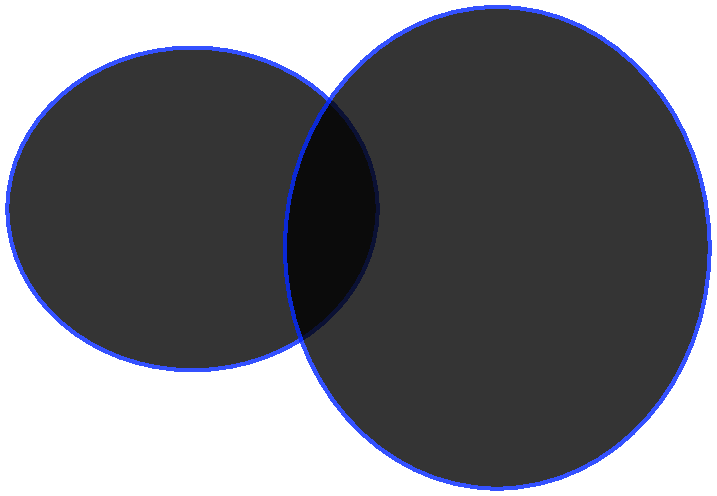
\includegraphics[scale=0.5]{circles.pdf}
		\caption{A sample circles graphic (.pdf format).}
		\label{fig:circles}
	\end{figure}

	This sample document contains examples of \textbf{.png} files to be displayable with \LaTeX.
	Usage of this type of figure element is seen in Figure~\ref{fig:star}.
	
	\begin{figure}
		\centering
		
\includegraphics[scale=0.5]{star.png}
		\caption{A sample star graphic (.png format).}
		\label{fig:star}
	\end{figure}

	As was the case with tables, you may want a figure
that spans two columns.
	To do this, and still to
ensure proper ``floating'' placement of tables, use the environment
\textbf{figure*} to enclose the figure and its caption.
	
	\begin{figure*}
		\centering
		
\includegraphics[scale=0.8]{spin.png}
		\caption{A sample spin graphic with a span.}
		\label{fig:spin}
	\end{figure*}
	
	\section{Conclusions}
	
	This paragraph will end the body of this sample document.
	Remember that you might still have Acknowledgments or
Appendices; brief samples of these
follow.
	There is still the Bibliography to deal with; and
we will make a disclaimer about that here: with the exception
of the reference to the \LaTeX\ book, the citations in
this paper are to articles which have nothing to
do with the present subject and are used as
examples only.
	
	\section{Acknowledgments}
	
	This section is optional; it is a location for you
to acknowledge grants, funding, editing assistance and
what have you.
	In the present case, for example, the
authors would like to thank Klemen Berkovič for
his help in codifying this \textit{Author's Guide}
and the \textbf{.cls} and \textbf{.tex} files that it describes.

	\bibliography{references}
	
\end{document}
